\documentclass[a4paper,12pt]{article}
\usepackage{standalone}
\usepackage{amsmath} % Package for advanced math typesetting



% Basic
\usepackage[T1]{fontenc}
\usepackage[utf8]{inputenc}
\usepackage{titlesec}
\titleformat{\section}
  {\normalfont\fontsize{14}{15}\bfseries}{\thesection}{1em}{}
\titleformat{\subsection}
  {\normalfont\fontsize{12}{15}\bfseries}{\thesubsection}{1em}{}

% Changes sections from 1.1 to 1.a
\renewcommand{\thesubsection}{\thesection.\alph{subsection}}

% ------------------------------------------------------------ %

% Packages
\RequirePackage{tcolorbox}
\usepackage{amsmath, amsthm, amssymb}
\usepackage{blindtext}
\usepackage{enumitem}
\usepackage{extramarks}
\usepackage{fancyhdr}
\usepackage[margin=1in]{geometry}
\usepackage{graphicx}
\usepackage{hyperref}
\usepackage{indentfirst}
\usepackage{listings}
\usepackage{mathrsfs}
\usepackage{mdframed}
\usepackage{multicol, multirow}
\usepackage{needspace, setspace}
\usepackage{paracol}
\usepackage{pgf, pgfplots}
\usepackage{tikz}
\usetikzlibrary{patterns}
\usepackage{silence}
\usepackage{xcolor}
\usepackage{bookmark}
\setlength{\parindent}{0pt}
\usetikzlibrary{patterns}
% \usepackage{subcaption}
\usetikzlibrary{decorations.pathreplacing}
\usepackage{caption}
\usepackage{subcaption}
\usepackage{xcolor}
\definecolor{maroon}{RGB}{128, 0, 0}
% ------------------------------------------------------------ %

% Spacings
\newcommand{\n}{\vspace{3mm}} % Context spacing
\newcommand{\s}{\vspace{1mm}} % Equation spacing
\newcommand{\m}{\vspace{-3mm}} % Reverse context spacing
\newcommand{\propdisp}{\pagebreak} % Proper display page break
\newcommand{\br}{\n\\\n}

% Wordings
\newcommand{\ans}[1][zb]{{\color{#1}\textit{Answer. }\hspace{3mm}}} % Answer
\newcommand{\arl}[1][zr]{{\color{#1}$\brr{\Leftarrow}$\hspace{3mm}}} % Left arrow
\newcommand{\arr}[1][zr]{{\color{#1}$\brr{\Rightarrow}$\hspace{3mm}}} % Right arrow
\newcommand{\cse}[2][zr]{{\color{#1}\textit{Case #2: }\hspace{1mm}}} % Case
\newcommand{\clm}[2][zr]{{\color{#1}$\vdash_{#2}$\hspace{1mm}}} % Claim
\newcommand{\prf}[1][zr]{{\color{#1}\textit{Proof. }\hspace{3mm}}} % Proof
\newcommand{\prt}[2][a]{\hspace{-2mm}{\color{#2}\textit{Part (#1) }}\hspace{1mm}} % Part
\newcommand{\prtc}[2][a]{\hspace{2mm}\prt[#1]{#2}} % Continued part

\newcommand{\rdft}[1][\sct]{{\color{zg}\textit{Definition #1}}} % Refer definition
\newcommand{\rexm}[1][\sct]{{\color{zb}\textit{Example #1}}} % Refer example
\newcommand{\rfig}[1][\sct]{{\color{zy}\textit{Figure #1}}} % Refer figure
\newcommand{\rpst}[1][\sct]{{\color{zr}\textit{Proposition #1}}} % Refer proposition
\newcommand{\rthm}[1][\sct]{{\color{zr}\textit{Theorem #1}}} % Refer theorem

\newcommand{\sct}{\thesection.\thescount} % Counter
\newcommand{\sctr}[2][0]{\the\numexpr\value{section}-#1\relax.\the\numexpr\value{scount}-#2\relax} % Relative counter

% Equations
\newcommand{\C}{\mathbb{C}} % Complex
\newcommand{\F}{\mathbb{F}} % Field
\newcommand{\I}{\mathbb{I}} % Irrational
\newcommand{\N}{\mathbb{N}} % Natural
\newcommand{\Q}{\mathbb{Q}} % Rational
\newcommand{\R}{\mathbb{R}} % Real
\newcommand{\Z}{\mathbb{Z}} % Integer

\newcommand{\GL}{\mathrm{GL}} % General linear group
\newcommand{\SL}{\mathrm{SL}} % Special linear group

\newcommand{\abs}[1]{\left| #1\right|} % Absolute
\newcommand{\bra}[1]{\left\langle #1\right\rangle} % Angled brackets
\newcommand{\brc}[1]{\left\{ #1\right\}} % Curly brackets
\newcommand{\brr}[1]{\left( #1\right)} % Round brackets
\newcommand{\brs}[1]{\left[ #1\right]} % Square brackets
\newcommand{\cond}[1]{\left. #1\right|} % Condition with right bar
\newcommand{\diff}{\,\mathrm{d}} % Differential
\newcommand{\erm}[1]{\;\;\;\;\text{#1}} % Equation remarks
\newcommand{\nrm}[1]{\left\| #1\right\|} % Norm
\newcommand{\srm}{\,\mid\,} % Set remarks

% Math operators
\let\Im\relax
\let\Re\relax

\DeclareMathOperator{\Im}{Im} % Imaginary function
\DeclareMathOperator{\Re}{Re} % Real function

% ------------------------------------------------------------ %

% Colours
\definecolor{gr}{RGB}{120, 120, 120} % Grey
\definecolor{zb}{RGB}{0, 38, 77} % Blue
\definecolor{zg}{RGB}{0, 77, 51} % Green
\definecolor{zp}{RGB}{51, 0, 77} % Purple
\definecolor{zr}{RGB}{77, 0, 38} % Red
\definecolor{zy}{RGB}{77, 64, 0} % Yellow

% Graphing
\usetikzlibrary{arrows}
\usetikzlibrary{calc}
\usetikzlibrary{patterns}
\pgfplotsset{compat=1.15}

% ------------------------------------------------------------ %

% Remark
\newcommand{\remark}[1]{
  \noindent\textbf{Remarks}
  
  \begin{nlist}
    \item Context of this document is based on university course \textit{\gettitle} from \textit{Department of Mathematics, The Chinese University of Hong Kong}. The original source can be found at \url{https://www.math.cuhk.edu.hk/course}. The author does not own the source.
    \item This document is assumed unavailable for unauthorized parties that have not attended the university course. It is prohibited to share, including distributing or copying this document to unauthorized parties in any means for any non-academic purpose.
    \item Context of this doucment may not be completely accurate. The author assumes no responsibility or liability for any errors or omissions in the context of this document.
    \item This document is under license CC-BY-SA 4.0. It is allowed to make any editions on this document, as long as terms of the license is not violated.
    #1
  \end{nlist}
}

% Prerequisites
\newenvironment{prereq}{
  \noindent \textbf{Prerequisites}\n

  This course requires prerequisites of
}{
  \n
}

% Reference list
\newenvironment{reflist}{
  \begin{alist}
    \item Course material from various professors associated to \textit{\gettitle}
}{
  \end{alist}
}

% ------------------------------------------------------------ %

% Environments
\newcounter{scount}[section] % Counter

\newenvironment{crl}{ % Corollary
  \parindent 0pt
  \begin{siderule}[linecolor=zr]{\color{zr}\textit{Corollary. }}
}{
  \end{siderule}
}

\newenvironment{cmt}{ % Comment
  \parindent 0pt
  \begin{siderule}[linecolor=zp]{\color{zp}\textit{Comment. }}
}{
  \end{siderule}
}

\newenvironment{dft}{ % Definition
  \parindent 0pt
  \refstepcounter{scount}
  \begin{siderule}[linecolor=zg]{\color{zg}\textit{Definition \sct. }}
}{
  \end{siderule}
}
\newenvironment{lem}{ % Lemma
  \parindent 0pt
  \refstepcounter{scount}
  \begin{siderule}[linecolor=zg]{\color{zg}\textit{Lemma \sct. }}
}{
  \end{siderule}
}

\newenvironment{exm}{ % Example
  \parindent 0pt
  \refstepcounter{scount}
  \begin{siderule}[linecolor=zb]{\color{zb}\textit{Example \sct. }}
}{
  \end{siderule}
}

\newenvironment{fig}{ % Figure
  \parindent 0pt
  \refstepcounter{scount}
  \begin{siderule}[linecolor=zy]{\color{zy}\textit{Figure \sct. }}\n
  
}{
  \end{siderule}
}

\newenvironment{prv}{ % Proof
  \parindent 0pt
  \begin{siderule}[linecolor=zr]\prf
}{
  \end{siderule}
}

\newenvironment{pst}{ % Proposition
  \parindent 0pt
  \refstepcounter{scount}
  \begin{siderule}[linecolor=zr]{\color{zr}\textit{Proposition \sct. }}
}{
  \end{siderule}
}

\newenvironment{tcn}{ % Technique
  \parindent 0pt
  \begin{siderule}[linecolor=zp]{\color{zp}\textit{Technique. }}
}{
  \end{siderule}
}

\newenvironment{thm}{ % Theorem
  \parindent 0pt
  \refstepcounter{scount}
  \begin{siderule}[linecolor=zr]{\color{zr}\textit{Sætning \sct. }}
}{
  \end{siderule}
}

\newenvironment{rmatrix}{ % Matrix in round brackets
  \left(\begin{matrix}
}{
  \end{matrix}\right)
}

\newenvironment{alist}{ % Alphabetical list
  \begin{enumerate}[label=(\alph*)]
}{
  \end{enumerate}
}

\newenvironment{Alist}{ % Capitalized alphabetical list
  \begin{enumerate}[label=(\Alph*)]
}{
  \end{enumerate}
}

\newenvironment{nlist}{ % Number list
  \begin{enumerate}[label=(\arabic*)]
}{
  \end{enumerate}
}

\newenvironment{plist}{ % Point list
  \begin{itemize}
}{
  \end{itemize}
}

\newenvironment{rlist}{ % Roman list
  \begin{enumerate}[label=(\roman*)]
}{
  \end{enumerate}
}

\newmdenv[ % Siderule line
  topline=false,
  bottomline=false,
  rightline=false,
  rightmargin=0
]{siderule}


% ------------------------------------------------------------ %
% Warning filters
\WarningFilter{mdframed}{You got a bad break}
\hfuzz=8pt


% Load required packages
\usepackage{tcolorbox}
% ------------------------------------------------------------ %

% Code

\usepackage{amsmath}
\usepackage{graphicx}
\definecolor{bluekeywords}{rgb}{0.13,0.13,1}
\definecolor{greencomments}{rgb}{0,0.5,0}
\definecolor{redstrings}{rgb}{0.9,0,0}
\definecolor{bgcolor}{rgb}{0.95,0.94,0.94}
\usepackage{listings}
\usepackage{upquote}
\usepackage{xcolor}

\lstdefinelanguage{Python}
{
  keywords={typeof, null, catch, switch, in, int, str, float, self},
  keywordstyle=\color{ForestGreen}\bfseries,
  ndkeywords={boolean, throw, import},
  ndkeywords={return, class, if ,elif, endif, while, do, else, True, False , catch, def},
  ndkeywordstyle=\color{BrickRed}\bfseries,
  identifierstyle=\color{black},
  sensitive=false,
  comment=[l]{\#},
  morecomment=[s]{/*}{*/},
  commentstyle=\color{purple}\ttfamily,
  stringstyle=\color{red}\ttfamily,
}

\lstset
{ %Formatting for code in appendix
    language=Python,
    numbers=left,
    stepnumber=1,
    showstringspaces=false,
    tabsize=1,
    breaklines=true,
    breakatwhitespace=false,
    backgroundcolor=\color{bgcolor},  % Background color
    basicstyle=\ttfamily\footnotesize, % Code font size and style
    frame=single,                    % Adds a frame around the code
    rulecolor=\color{bgcolor},       % Frame color
    breaklines=true,                 % Breaks long lines
}
 % Assuming these files exist and are correctly referenced
\graphicspath{ {../../pictures/IDMA/IDMA_4a}} % Assuming a pictures folder has been made and is correctly referenced

% \renewcommand{\thesection}{5.\arabic{section}} % Substitue 5. for any number

% Changes sections from 1.1 to 1.a
\renewcommand{\thesubsection}{\thesection.\alph{subsection}}

\begin{document}
% \includepdf[pages=-]{../../pictures/forside}

\title{Københavns Universitet\\
Introduktion til diskret matematik og algoritmer - Problem set 3}
\author{Victor Vangkilde Jørgensen}
\makeatletter
\let\getauthor\@author
\let\gettitle\@title
\makeatother
\maketitle
\thispagestyle{empty}
\n\n
 % Assuming this file contains the cover page setup

\pagebreak
\pagestyle{empty}
\tableofcontents
\pagebreak
\pagestyle{fancy}
\fancyhf{}
\setlength{\headheight}{15.2pt}
\renewcommand{\footrulewidth}{0.4pt}
% \fancyhead[R]{\nouppercase \lastrightmark}
\fancyfoot[L]{\gettitle}
\fancyfoot[R]{\thepage}
 % Assuming this file contains the header setup
\maketitle % This command will actually insert the title into the document



\section[Question 1]{}
\begin{figure}[H]
    \centering
    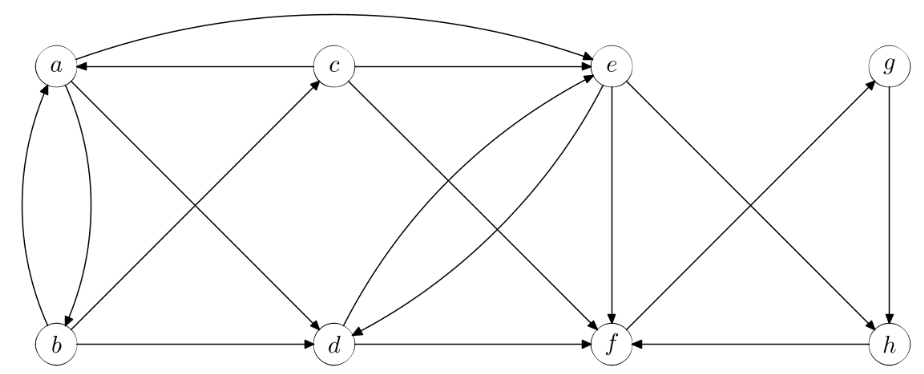
\includegraphics[width=0.9\textwidth]{1.png}
    \caption{Directed graph $G$ for which to compute strongly connected components in Problem 1a.}
\end{figure}

\subsection[]{}
Vi opskriver vores directed graph som en adjacency list representation i lexicographic order:
\[
\begin{aligned}
&a \rightarrow (b, d, e)\\
&b \rightarrow (a, c, d)\\
&c \rightarrow (a, e, f)\\
&d \rightarrow (e, f)\\
&e \rightarrow (d, f, h)\\
&f \rightarrow (g)\\
&g \rightarrow (h)\\
&h \rightarrow (f)\\
\end{aligned}
\]


\begin{figure}[H]
    \centering
    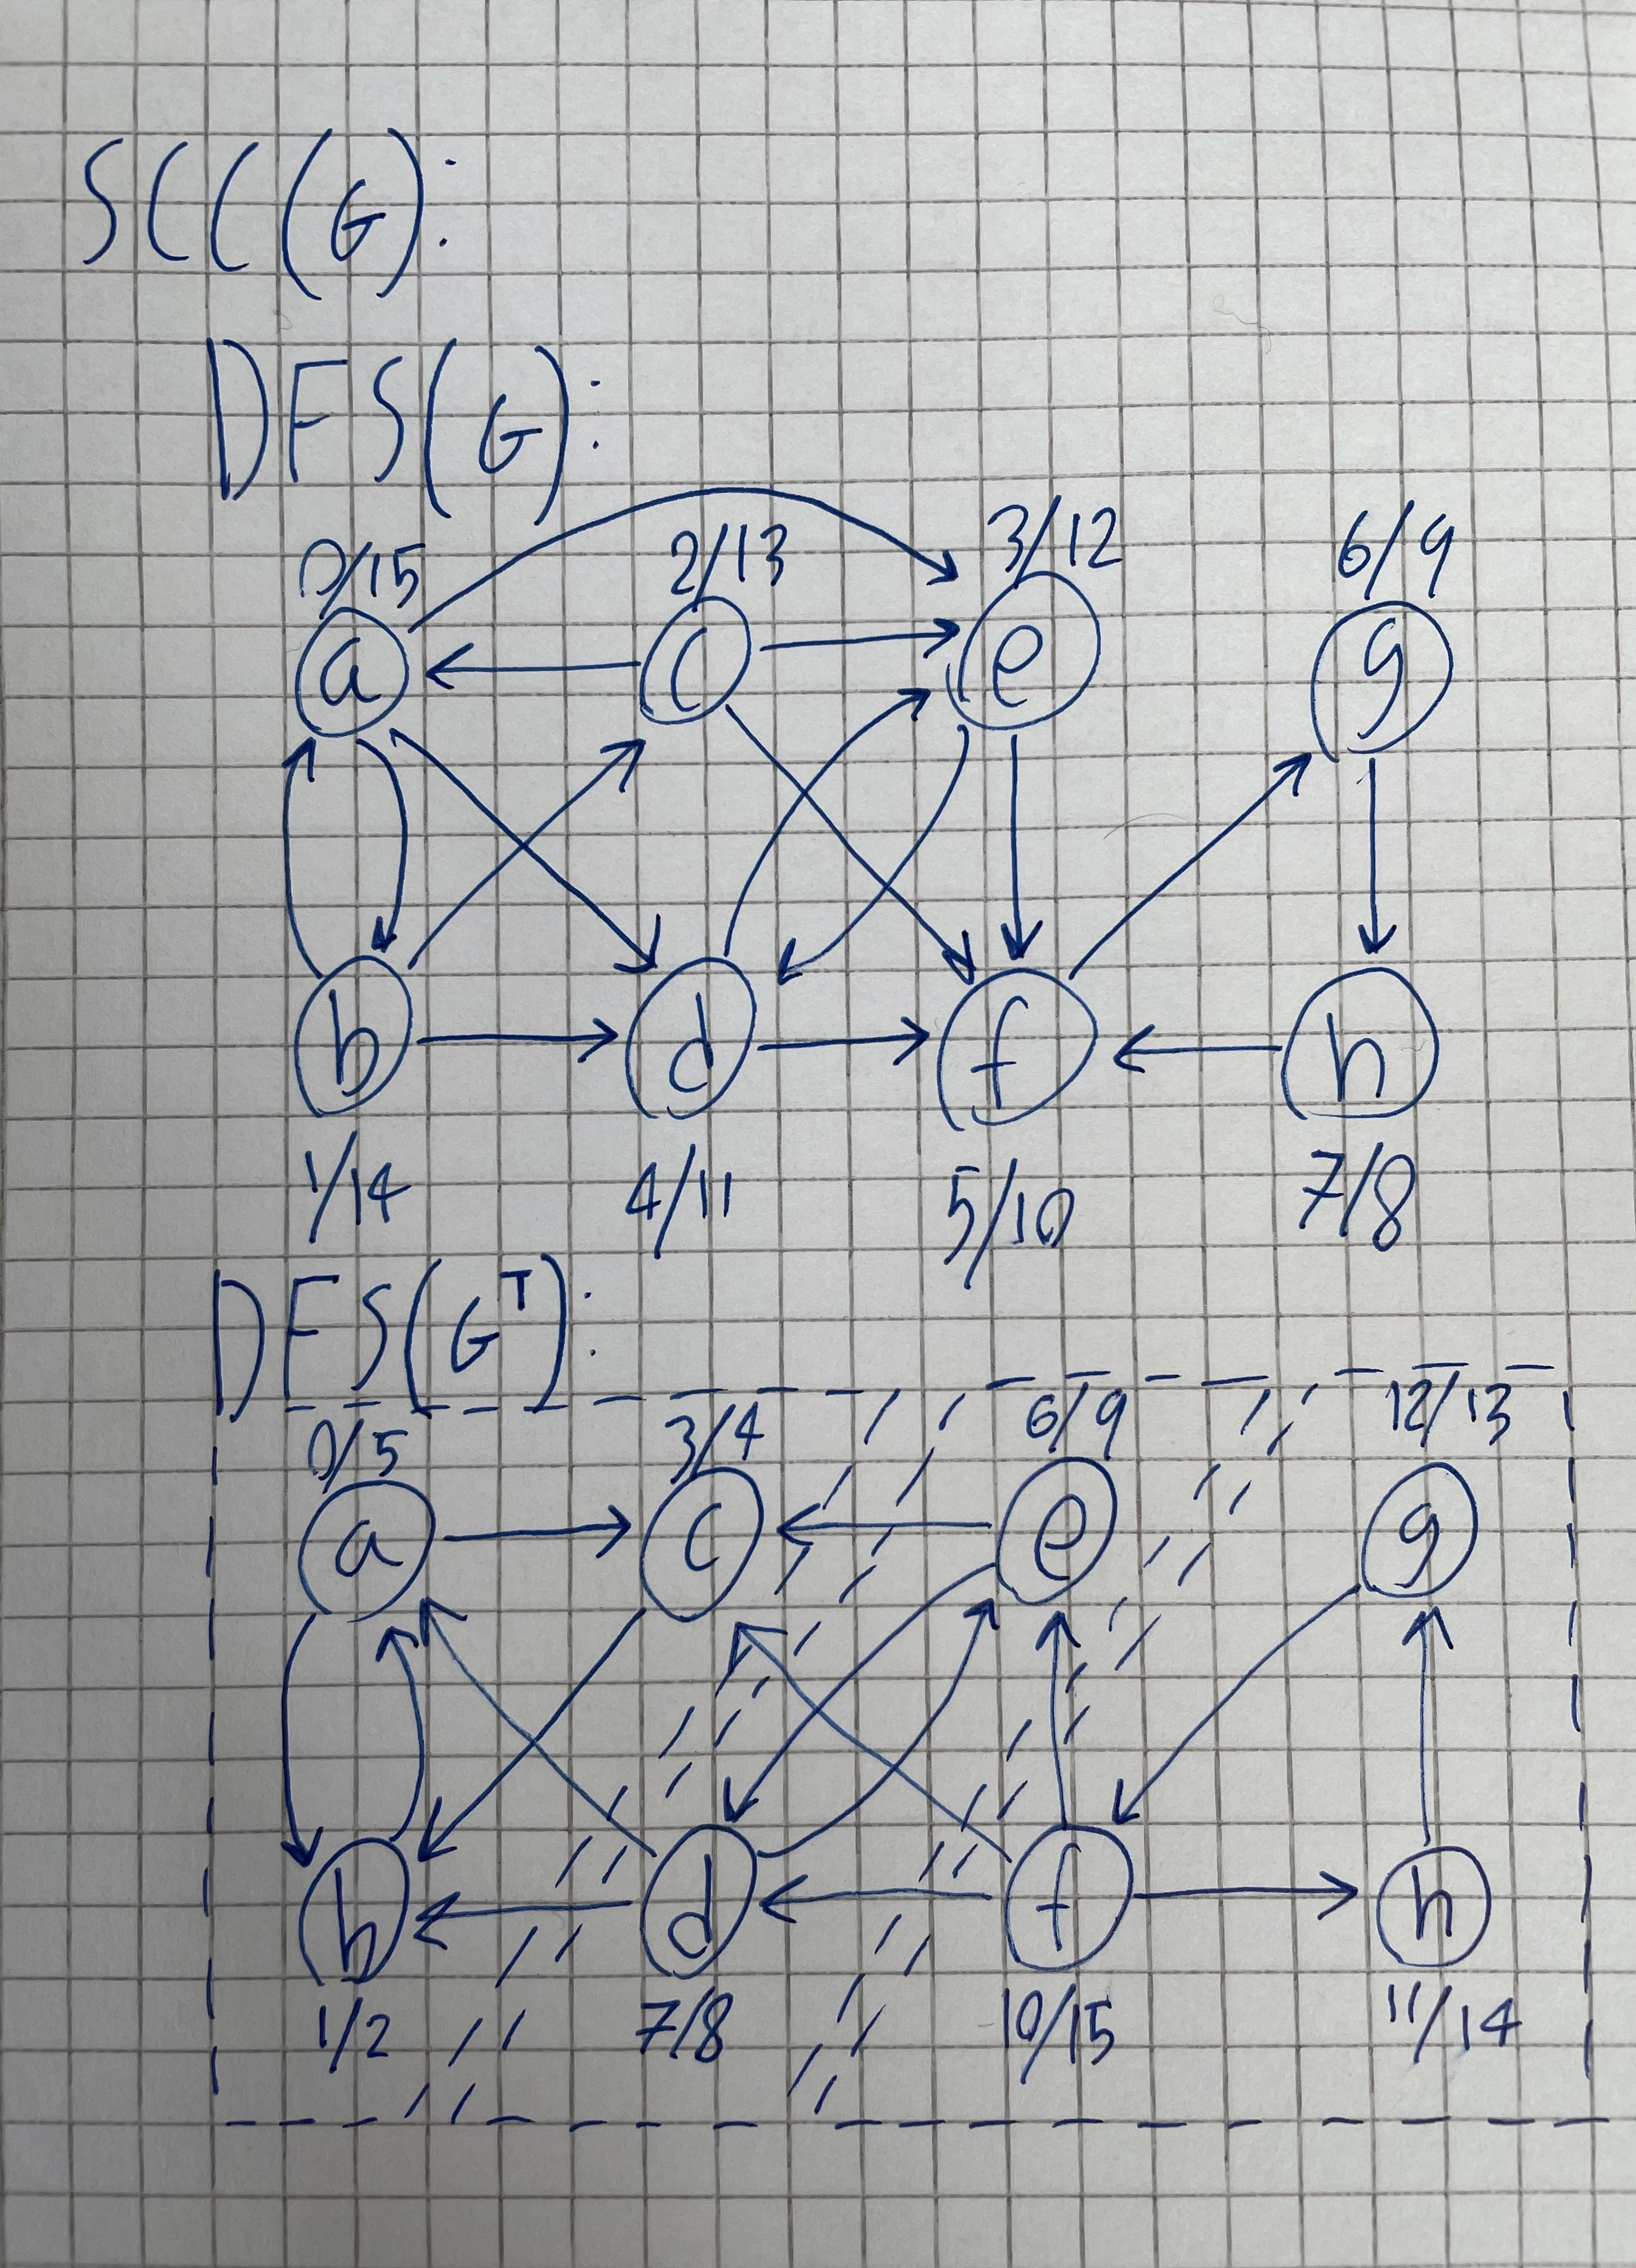
\includegraphics[width=1\textwidth]{SCC.jpg}
    \caption{Gennemgang af $SCC(G)$.}
\end{figure}

\subsection[]{}



\section[Question 2]{}
\begin{figure}[H]
    \centering
    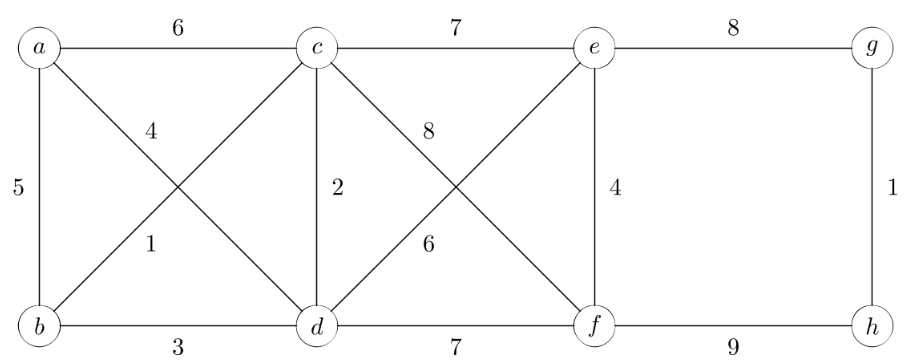
\includegraphics[width=1\textwidth]{2.png}
    \caption{Undirected graph for which to compute minimum spanning tree in Problem 2a.}
\end{figure}
\subsection[]{}

Vi har følgende vertices:
\begin{figure}[H]
    \centering
    \begin{tikzpicture}[scale=2]
        \node[red, circle, draw] (a) at (0,2) {$a$};
        \node[red, circle, draw] (b) at (0,0) {$b$};
        \node[red, circle, draw] (c) at (2,2) {$c$};
        \node[red, circle, draw] (d) at (2,0) {$d$};
        \node[red, circle, draw] (e) at (4,2) {$e$};
        \node[red, circle, draw] (f) at (4,0) {$f$};
        \node[red, circle, draw] (g) at (6,2) {$g$};
        \node[red, circle, draw] (h) at (6,0) {$h$};
        % \draw (a) -- (c) node[midway, above] {6};
        % \draw (a) -- (b) node[midway, left] {5};
        % \draw (a) -- (d) node[midway, above left, yshift=10pt] {4};
        % \draw (b) -- (d) node[midway, below] {3};
        % \draw (b) -- (c) node[midway, below left, yshift=11pt] {1};
        % \draw (c) -- (d) node[midway, right] {2};
        % \draw (c) -- (e) node[midway, above] {7};
        % \draw (c) -- (f) node[midway, above left, , yshift=10pt] {8};
        % \draw (e) -- (f) node[midway, right] {4};
        % \draw (e) -- (g) node[midway, above] {8};
        % \draw (f) -- (h) node[midway, below] {9};
        % \draw (g) -- (h) node[midway, right] {1};
        % \draw (d) -- (f) node[midway, below] {7};
        % \draw (d) -- (e) node[midway, below left, yshift=-10pt] {6};
    \end{tikzpicture}
    \caption*{}
\end{figure}
Som vi kan skrive op som subsets med alle connectede vertices. I begyndelsen har vi bare:
\[\{a\},\{b\},\{c\},\{d\},\{e\},\{f\},\{g\},\{h\}\]

Vi ser, at $(b,c)\in E$ har lavest vægt, sammen med $(g,h)\in E$. I lexicographic order vælger vi først $(b,c)\in E$.\\
$(b,c)\in E$ connecter kun ikke-connetede vertices sammen, da disse er de eneste elementer i deres subsets, så vi connecter dem.
\begin{figure}[H]
    \centering
    \begin{tikzpicture}[scale=2]
        \node[red, circle, draw] (a) at (0,2) {$a$};
        \node[green, circle, draw] (b) at (0,0) {$b$};
        \node[green, circle, draw] (c) at (2,2) {$c$};
        \node[red, circle, draw] (d) at (2,0) {$d$};
        \node[red, circle, draw] (e) at (4,2) {$e$};
        \node[red, circle, draw] (f) at (4,0) {$f$};
        \node[red, circle, draw] (g) at (6,2) {$g$};
        \node[red, circle, draw] (h) at (6,0) {$h$};
        % \draw (a) -- (c) node[midway, above] {6};
        % \draw (a) -- (b) node[midway, left] {5};
        % \draw (a) -- (d) node[midway, above left, yshift=10pt] {4};
        % \draw (b) -- (d) node[midway, below] {3};
        \draw (b) -- (c) node[midway, below left, yshift=11pt] {1};
        % \draw (c) -- (d) node[midway, right] {2};
        % \draw (c) -- (e) node[midway, above] {7};
        % \draw (c) -- (f) node[midway, above left, , yshift=10pt] {8};
        % \draw (e) -- (f) node[midway, right] {4};
        % \draw (e) -- (g) node[midway, above] {8};
        % \draw (f) -- (h) node[midway, below] {9};
        % \draw (g) -- (h) node[midway, right] {1};
        % \draw (d) -- (f) node[midway, below] {7};
        % \draw (d) -- (e) node[midway, below left, yshift=-10pt] {6};
    \end{tikzpicture}
    \caption*{}
\end{figure}
Nu har vi nogle nye connectede vertices, så vi samler deres subsets:
\[\{b,c\},\{a\},\{d\},\{e\},\{f\},\{g\},\{h\}\]

Vi kigger derefter på $(g,h)\in E$, da denne edge er den næste i acending order af weight.\\
$(g,h)\in E$ connecter kun ikke-connetede vertices sammen, da disse vertices er i forskellige subsets, så vi connecter dem.
\begin{figure}[H]
    \centering
    \begin{tikzpicture}[scale=2]
        \node[red, circle, draw] (a) at (0,2) {$a$};
        \node[green, circle, draw] (b) at (0,0) {$b$};
        \node[green, circle, draw] (c) at (2,2) {$c$};
        \node[red, circle, draw] (d) at (2,0) {$d$};
        \node[red, circle, draw] (e) at (4,2) {$e$};
        \node[red, circle, draw] (f) at (4,0) {$f$};
        \node[green, circle, draw] (g) at (6,2) {$g$};
        \node[green, circle, draw] (h) at (6,0) {$h$};
        % \draw (a) -- (c) node[midway, above] {6};
        % \draw (a) -- (b) node[midway, left] {5};
        % \draw (a) -- (d) node[midway, above left, yshift=10pt] {4};
        % \draw (b) -- (d) node[midway, below] {3};
        \draw (b) -- (c) node[midway, below left, yshift=11pt] {1};
        % \draw (c) -- (d) node[midway, right] {2};
        % \draw (c) -- (e) node[midway, above] {7};
        % \draw (c) -- (f) node[midway, above left, , yshift=10pt] {8};
        % \draw (e) -- (f) node[midway, right] {4};
        % \draw (e) -- (g) node[midway, above] {8};
        % \draw (f) -- (h) node[midway, below] {9};
        \draw (g) -- (h) node[midway, right] {1};
        % \draw (d) -- (f) node[midway, below] {7};
        % \draw (d) -- (e) node[midway, below left, yshift=-10pt] {6};
    \end{tikzpicture}
    \caption*{}
\end{figure}
Nu har vi nogle nye connectede vertices, så vi samler deres subsets:
\[\{b,c\},\{g,h\},\{a\},\{d\},\{e\},\{f\}\]

Vi kigger derefter på $(c,d)\in E$, da denne edge er den næste i acending order af weight.\\
$(c,d)\in E$ connecter $d$, som ikke er connected gennem andre edges, da disse vertices er i forskellige subsets, så vi connecter dem.
\begin{figure}[H]
    \centering
    \begin{tikzpicture}[scale=2]
        \node[red, circle, draw] (a) at (0,2) {$a$};
        \node[green, circle, draw] (b) at (0,0) {$b$};
        \node[green, circle, draw] (c) at (2,2) {$c$};
        \node[green, circle, draw] (d) at (2,0) {$d$};
        \node[red, circle, draw] (e) at (4,2) {$e$};
        \node[red, circle, draw] (f) at (4,0) {$f$};
        \node[green, circle, draw] (g) at (6,2) {$g$};
        \node[green, circle, draw] (h) at (6,0) {$h$};
        % \draw (a) -- (c) node[midway, above] {6};
        % \draw (a) -- (b) node[midway, left] {5};
        % \draw (a) -- (d) node[midway, above left, yshift=10pt] {4};
        % \draw (b) -- (d) node[midway, below] {3};
        \draw (b) -- (c) node[midway, below left, yshift=11pt] {1};
        \draw (c) -- (d) node[midway, right] {2};
        % \draw (c) -- (e) node[midway, above] {7};
        % \draw (c) -- (f) node[midway, above left, , yshift=10pt] {8};
        % \draw (e) -- (f) node[midway, right] {4};
        % \draw (e) -- (g) node[midway, above] {8};
        % \draw (f) -- (h) node[midway, below] {9};
        \draw (g) -- (h) node[midway, right] {1};
        % \draw (d) -- (f) node[midway, below] {7};
        % \draw (d) -- (e) node[midway, below left, yshift=-10pt] {6};
    \end{tikzpicture}
    \caption*{}
\end{figure}
Nu har vi nogle nye connectede vertices, så vi samler deres subsets:
\[\{b,c,d\},\{g,h\},\{a\},\{e\},\{f\}\]

Vi kigger derefter på $(b,d)\in E$, da denne edge er den næste i acending order af weight.\\
$b$ og $d$, er allerede connected gennem andre edges, da de er i samme subset, så vi ignorerer den edge.\\
Vi kigger derefter på $(a,d)\in E$, da denne edge er den næste i acending order af weight.\\
$(a,d)\in E$ connecter $a$, som ikke er connected gennem andre edges, da disse vertices er i forskellige subsets, så vi connecter dem.
\begin{figure}[H]
    \centering
    \begin{tikzpicture}[scale=2]
        \node[green, circle, draw] (a) at (0,2) {$a$};
        \node[green, circle, draw] (b) at (0,0) {$b$};
        \node[green, circle, draw] (c) at (2,2) {$c$};
        \node[green, circle, draw] (d) at (2,0) {$d$};
        \node[red, circle, draw] (e) at (4,2) {$e$};
        \node[red, circle, draw] (f) at (4,0) {$f$};
        \node[green, circle, draw] (g) at (6,2) {$g$};
        \node[green, circle, draw] (h) at (6,0) {$h$};
        % \draw (a) -- (c) node[midway, above] {6};
        % \draw (a) -- (b) node[midway, left] {5};
        \draw (a) -- (d) node[midway, above left, yshift=11pt] {4};
        % \draw (b) -- (d) node[midway, below] {3};
        \draw (b) -- (c) node[midway, below left, yshift=-11pt] {1};
        \draw (c) -- (d) node[midway, right] {2};
        % \draw (c) -- (e) node[midway, above] {7};
        % \draw (c) -- (f) node[midway, above left, , yshift=10pt] {8};
        % \draw (e) -- (f) node[midway, right] {4};
        % \draw (e) -- (g) node[midway, above] {8};
        % \draw (f) -- (h) node[midway, below] {9};
        \draw (g) -- (h) node[midway, right] {1};
        % \draw (d) -- (f) node[midway, below] {7};
        % \draw (d) -- (e) node[midway, below left, yshift=-10pt] {6};
    \end{tikzpicture}
    \caption*{}
\end{figure}
Nu har vi nogle nye connectede vertices, så vi samler deres subsets:
\[\{a,b,c,d\},\{g,h\},\{e\},\{f\}\]

Vi kigger derefter på $(e,f)\in E$, da denne edge er den næste i acending order af weight.\\
$(e,f)\in E$ connecter kun ikke-connetede vertices sammen, da disse vertices er i forskellige subsets, så vi connecter dem.
\begin{figure}[H]
    \centering
    \begin{tikzpicture}[scale=2]
        \node[green, circle, draw] (a) at (0,2) {$a$};
        \node[green, circle, draw] (b) at (0,0) {$b$};
        \node[green, circle, draw] (c) at (2,2) {$c$};
        \node[green, circle, draw] (d) at (2,0) {$d$};
        \node[green, circle, draw] (e) at (4,2) {$e$};
        \node[green, circle, draw] (f) at (4,0) {$f$};
        \node[green, circle, draw] (g) at (6,2) {$g$};
        \node[green, circle, draw] (h) at (6,0) {$h$};
        % \draw (a) -- (c) node[midway, above] {6};
        % \draw (a) -- (b) node[midway, left] {5};
        \draw (a) -- (d) node[midway, above left, yshift=11pt] {4};
        % \draw (b) -- (d) node[midway, below] {3};
        \draw (b) -- (c) node[midway, below left, yshift=-11pt] {1};
        \draw (c) -- (d) node[midway, right] {2};
        % \draw (c) -- (e) node[midway, above] {7};
        % \draw (c) -- (f) node[midway, above left, , yshift=10pt] {8};
        \draw (e) -- (f) node[midway, right] {4};
        % \draw (e) -- (g) node[midway, above] {8};
        % \draw (f) -- (h) node[midway, below] {9};
        \draw (g) -- (h) node[midway, right] {1};
        % \draw (d) -- (f) node[midway, below] {7};
        % \draw (d) -- (e) node[midway, below left, yshift=-10pt] {6};
    \end{tikzpicture}
    \caption*{}
\end{figure}
Nu har vi nogle nye connectede vertices, så vi samler deres subsets:
\[\{a,b,c,d\},\{e,f\},\{g,h\}\]

Vi kigger derefter på $(a,b)\in E$, da denne edge er den næste i acending order af weight.\\
$a$ og $b$, er allerede connected gennem andre edges, da de er i samme subset, så vi ignorerer den edge.\\
Vi kigger derefter på $(a,c)\in E$, da denne edge er den næste i acending order af weight.\\
$a$ og $c$, er allerede connected gennem andre edges, da de er i samme subset, så vi ignorerer den edge.\\
Vi kigger derefter på $(d,e)\in E$, da denne edge er den næste i acending order af weight.\\
$(d,e)\in E$ connecter både $e$ og $f$, som ikke er connected gennem andre edges, da disse vertices er i forskellige subsets, så vi connecter dem.
\begin{figure}[H]
    \centering
    \begin{tikzpicture}[scale=2]
        \node[green, circle, draw] (a) at (0,2) {$a$};
        \node[green, circle, draw] (b) at (0,0) {$b$};
        \node[green, circle, draw] (c) at (2,2) {$c$};
        \node[green, circle, draw] (d) at (2,0) {$d$};
        \node[green, circle, draw] (e) at (4,2) {$e$};
        \node[green, circle, draw] (f) at (4,0) {$f$};
        \node[green, circle, draw] (g) at (6,2) {$g$};
        \node[green, circle, draw] (h) at (6,0) {$h$};
        % \draw (a) -- (c) node[midway, above] {6};
        % \draw (a) -- (b) node[midway, left] {5};
        \draw (a) -- (d) node[midway, above left, yshift=11pt] {4};
        % \draw (b) -- (d) node[midway, below] {3};
        \draw (b) -- (c) node[midway, below left, yshift=-11pt] {1};
        \draw (c) -- (d) node[midway, right] {2};
        % \draw (c) -- (e) node[midway, above] {7};
        % \draw (c) -- (f) node[midway, above left, , yshift=10pt] {8};
        \draw (e) -- (f) node[midway, right] {4};
        % \draw (e) -- (g) node[midway, above] {8};
        % \draw (f) -- (h) node[midway, below] {9};
        \draw (g) -- (h) node[midway, right] {1};
        % \draw (d) -- (f) node[midway, below] {7};
        \draw (d) -- (e) node[midway, below left, yshift=10pt] {6};
    \end{tikzpicture}
    \caption*{}
\end{figure}
Nu har vi nogle nye connectede vertices, så vi samler deres subsets:
\[\{a,b,c,d,e,f\},\{g,h\}\]

Vi kigger derefter på $(c,e)\in E$, da denne edge er den næste i acending order af weight.\\
$c$ og $e$, er allerede connected gennem andre edges, da de er i samme subset, så vi ignorerer den edge.\\
Vi kigger derefter på $(d,f)\in E$, da denne edge er den næste i acending order af weight.\\
$d$ og $f$, er allerede connected gennem andre edges, da de er i samme subset, så vi ignorerer den edge.\\
Vi kigger derefter på $(c,f)\in E$, da denne edge er den næste i acending order af weight.\\
$c$ og $f$, er allerede connected gennem andre edges, da de er i samme subset, så vi ignorerer den edge.\\
Vi kigger derefter på $(e,g)\in E$, da denne edge er den næste i acending order af weight.\\
$(e,g)\in E$ connecter både $e$ og $g$, som ikke er connected gennem andre edges, da disse vertices er i forskellige subsets, så vi connecter dem.
\begin{figure}[H]
    \centering
    \begin{tikzpicture}[scale=2]
        \node[green, circle, draw] (a) at (0,2) {$a$};
        \node[green, circle, draw] (b) at (0,0) {$b$};
        \node[green, circle, draw] (c) at (2,2) {$c$};
        \node[green, circle, draw] (d) at (2,0) {$d$};
        \node[green, circle, draw] (e) at (4,2) {$e$};
        \node[green, circle, draw] (f) at (4,0) {$f$};
        \node[green, circle, draw] (g) at (6,2) {$g$};
        \node[green, circle, draw] (h) at (6,0) {$h$};
        % \draw (a) -- (c) node[midway, above] {6};
        % \draw (a) -- (b) node[midway, left] {5};
        \draw (a) -- (d) node[midway, above left, yshift=11pt] {4};
        % \draw (b) -- (d) node[midway, below] {3};
        \draw (b) -- (c) node[midway, below left, yshift=-11pt] {1};
        \draw (c) -- (d) node[midway, right] {2};
        % \draw (c) -- (e) node[midway, above] {7};
        % \draw (c) -- (f) node[midway, above left, , yshift=10pt] {8};
        \draw (e) -- (f) node[midway, right] {4};
        \draw (e) -- (g) node[midway, above] {8};
        % \draw (f) -- (h) node[midway, below] {9};
        \draw (g) -- (h) node[midway, right] {1};
        % \draw (d) -- (f) node[midway, below] {7};
        \draw (d) -- (e) node[midway, below left, yshift=10pt] {6};
    \end{tikzpicture}
    \caption*{}
\end{figure}
Nu har vi nogle nye connectede vertices, så vi samler deres subsets:
\[\{a,b,c,d,e,f,g,h\}\]

Vi ser, at vi har 7 edges og 8 vertices. Vi er dermed færdige, da antallet af edges svarer til antallet af vertices - 1, og alle vores vertices er i samme set, hvilket vil sige, at de er connected.


\subsection[]{}



\subsection[]{}



\subsection[]{}



\begin{figure}[H]
    \centering
    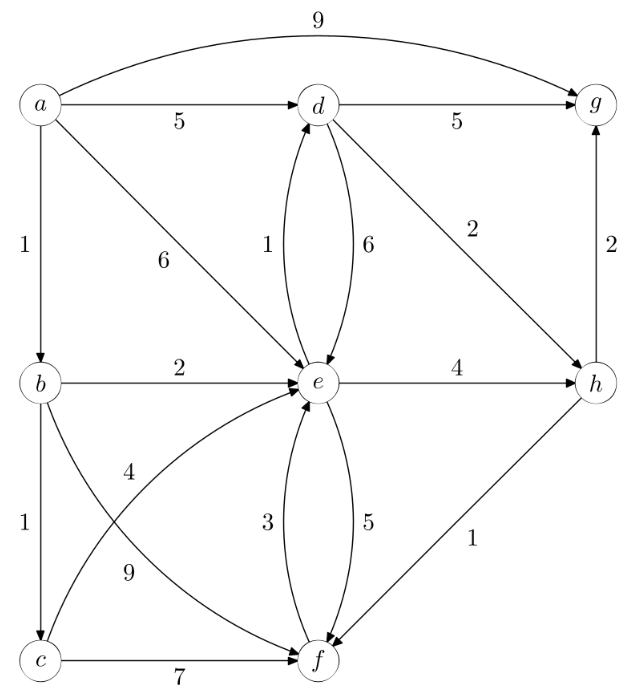
\includegraphics[width=0.8\textwidth]{3.png}
    \caption{Directed graph Dijkstra's algorithm in Problem 3a.}
\end{figure}
\section[Question 3]{}
\subsection[]{}

Jeg opskriver vores weighted directed graph som adjacency list representation $(vertex, weight)$:
\[
\begin{aligned}
&(a,0) \rightarrow ((b,1), (d,5), (e,6), (g,9))\\
&(b,0) \rightarrow ((c,1), (e,2), (f,9))\\
&(c,0) \rightarrow ((e,4), (f,7))\\
&(d,0) \rightarrow ((e,6), (g,5), (h,2))\\
&(e,0) \rightarrow ((d,1)(f,5), (h,4))\\
&(f,0) \rightarrow (e,3)\\
&(g,0) \rightarrow ()\\
&(h,0) \rightarrow (f,1)\\
\end{aligned}
\]

Udregning af distancer for $a's$ naboer:
\[
[(b,1),(d,5),(e,6),(g,9)]
\]
Vi opdaterer nu de laveste værdier i grafen:
\[
[(A,0),(b,1),(c,\infty),(d,5),(e,6),(f,\infty),(g,9),(h,\infty)]
\]
$a$ er nu besøgt, så det har jeg markeret ved at skrive $A$ i stedet.\\
\[
\begin{tikzpicture}[heap]
    \node {$(A,0)$}
        child{node{$(b,1)$}
            child{node{$(e,6)$} child{node{$(h,\infty)$}}} 
            child{node{$(g,9)$}}}
        child{node{$(d,5)$}
            child{node{$(c,\infty)$}} 
            child{node{$(f,\infty)$}}}
    ;
\end{tikzpicture}
\]

Vi ser, at $b$ er den ubesøgte vertex med kortest afstand fra $a.$\\
Udregning af nye distancer for $b's$ naboer:
\[
[(c,1+1),(e,1+2),(f,1+9)] = [(c,2),(e,3),(f,10)]
\]
Vi opdaterer nu de laveste værdier i grafen:
\[
[(A,0),(B,1),(c,2),(e,3),(d,5),(g,9),(f,10),(h,\infty)]
\]
$b$ er nu besøgt, så det har jeg markeret ved at skrive $B$ i stedet.\\

Vi ser, at $c$ er den ubesøgte vertex med kortest afstand fra $a$.\\
Udregning af nye distancer for $c's$ naboer:
\[
[(e,2+4),(f,2+7)] = [(e,6),(f,9)]
\]
Vi opdaterer nu de laveste værdier i grafen:
\[
[(A,0),(B,1),(C,2),(e,3),(d,5),(f,9),(g,9),(h,\infty)]
\]
$c$ er nu besøgt, så det har jeg markeret ved at skrive $C$ i stedet.\\

Vi ser, at $e$ er den ubesøgte vertex med kortest afstand fra $a$.\\
Udregning af nye distancer for $e's$ naboer:
\[
[(d,3+1),(f,3+5),(h,3+4)] = [(d,4),(f,8),(h,7)]
\]
Vi opdaterer nu de laveste værdier i grafen:
\[
[(A,0),(B,1),(C,2),(E,3),(d,4),(h,7),(f,8),(g,9)]
\]
$e$ er nu besøgt, så det har jeg markeret ved at skrive $E$ i stedet.\\

Vi ser, at $d$ er den ubesøgte vertex med kortest afstand fra $a$.\\
Udregning af nye distancer for $d's$ naboer:
\[
[(g,5+5),(h,5+5),(e,5+6)] = [(g,10),(h,10),(e,11)]
\]
Vi opdaterer nu de laveste værdier i grafen, men ser, at der ikke nogen kortere afstande:
\[
[(A,0),(B,1),(C,2),(E,3),(D,4),(h,7),(f,8),(g,9)]
\]
$d$ er nu besøgt, så det har jeg markeret ved at skrive $D$ i stedet.\\

Vi ser, at $h$ er den ubesøgte vertex med kortest afstand fra $a$.\\
Udregning af nye distancer for $h's$ naboer:
\[
[(f,7+1)] = [(f,8)]
\]
Vi opdaterer nu de laveste værdier i grafen, men ser, at der ikke nogen kortere afstande:
\[
[(A,0),(B,1),(C,2),(E,3),(D,4),(H,7),(f,8),(g,9)]
\]
$h$ er nu besøgt, så det har jeg markeret ved at skrive $H$ i stedet.\\

Vi ser, at $f$ er den ubesøgte vertex med kortest afstand fra $a$.\\
Udregning af nye distancer for $f's$ naboer:
\[
[(e,8+3)] = [(e,11)]
\]
Vi opdaterer nu de laveste værdier i grafen, men ser, at der ikke nogen kortere afstande:
\[
[(A,0),(B,1),(C,2),(E,3),(D,4),(H,7),(F,8),(g,9)]
\]
$f$ er nu besøgt, så det har jeg markeret ved at skrive $F$ i stedet.\\

Vi ser, at $g$ er den sidste ubesøgte vertex, og at $g$ ikke har nogen naboer.\\
\[
[(A,0),(B,1),(C,2),(E,3),(D,4),(H,7),(F,8),(G,9)]
\]
Vi markerer $g$ som besøgt med $G$.

\subsection[]{}



\subsection[]{}



\subsection[]{}



\end{document}